	\subsubsection{Temperatura de Burbuja}



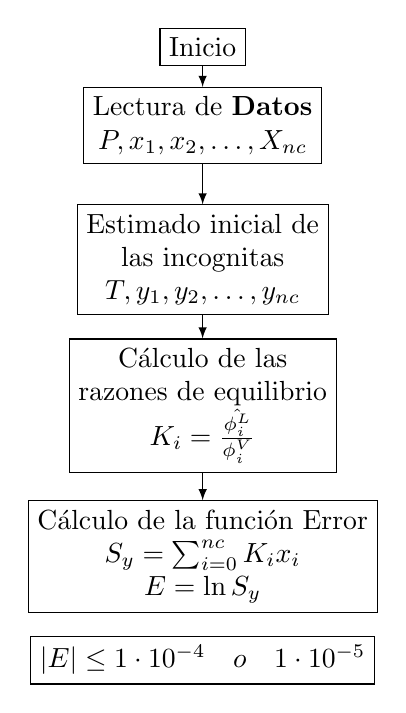
\begin{tikzpicture}[nodes={draw, fill=white,align=center},row sep=0.3cm,column sep=0.5cm] ]

\node(init){Inicio};
\node[below of=init] (lab)  {Lectura de \textbf{Datos} \\$P,x_1, x_2,\ldots, X_{nc}$};
\node[below of=lab,below](estim){Estimado inicial de\\ las incognitas\\$T,y_1,y_2,\ldots,y_{nc}$};
\node[below of=estim,below](relations){Cálculo de las\\ razones de equilibrio\\
$K_i = \frac{ \hat{\phi_i^L} }{ \phi_i^V}$};
\node[below of=relations,below = 0.2cm](error){Cálculo de la función Error\\$ S_y =\sum_{i=0}^{nc} K_i x_i $\\$ E = \ln{S_y} $};

\node[below of=error,below](criteria){$|E| \leq 1\cdot10^{-4}\quad \text{o} \quad  1\cdot 10^{-5}$};

\draw[-latex] (init)--(lab);
\draw[-latex] (lab)--(estim);
\draw[-latex] (estim)--(relations);
\draw[-latex] (relations)--(error);

\end{tikzpicture}
